\documentclass[11pt]{article}

\usepackage[margin=1in]{geometry}
\usepackage{amsmath,amssymb}
\usepackage{graphicx}
\usepackage{booktabs}
\usepackage{xcolor}
\usepackage{tikz}
\usetikzlibrary{arrows.meta,positioning,shapes.geometric,fit,backgrounds}
\usepackage[colorlinks=true,linkcolor=blue,citecolor=blue,urlcolor=blue]{hyperref}
\usepackage{caption}
\usepackage{float}
\usepackage{enumitem}

\newcommand{\Ubeta}{U_{\beta}}
\newcommand{\E}{\mathbb{E}}
\definecolor{good}{RGB}{22,163,74}
\definecolor{bad}{RGB}{220,38,38}
\definecolor{mid}{RGB}{37,99,235}

\title{\textbf{Entropic-Risk-Sensitive Jev}\\[2mm]
\large Risk-Aware Value Learning for Fast Decision Models\\ in Sequential Decision Making}
\author{Experimental report}
\date{\today}

\begin{document}
\maketitle

\begin{abstract}
A recent note argues that a fast ``System~1'' decision model such as
TypeSafe's \emph{Jev} (and its open analogue \texttt{choyiny/yev0-4b}) is, under a
terminal task reward, implicitly an \emph{action-value function}
$Q(s,a)=P(\text{success})$. That value is \emph{risk-neutral}: it ranks actions
purely by how \emph{likely} they are to succeed and is blind to \emph{how costly a
rare failure is}. This report develops \textbf{Entropic-Risk-Sensitive Jev}:
we replace the expectation in the value with the \emph{entropic (exponential-utility)
risk measure}, so the value reflects the full outcome distribution and penalises
rare-but-catastrophic failures. We build three purpose-made environments, derive
the risk-sensitive Bellman equations, and train value functions three ways:
exact value iteration, a risk-sensitive value head on frozen \texttt{yev0-4b}
features, and model-free deep RL (DQN, an exponential-utility DQN, and
QR-DQN with CVaR action selection). We evaluate every policy \emph{exactly} via
distributional policy evaluation against the mean, CVaR, entropic objective, and
catastrophe probabilities. The risk-sensitive controllers cut the major-catastrophe
rate by $5$--$40\times$ relative to the risk-neutral policy at a small cost in
mean return. Two routes make a real \texttt{yev0-4b} risk-sensitive: a value head
on its features, and --- most faithfully --- \textbf{LoRA fine-tuning of
\texttt{yev0-4b}'s own Choice probabilities with the blog's proper scoring rule},
which turns its native output from risk-blind ($\Ubeta=-55$, $4\%$ agreement with
the risk-sensitive oracle) into the \emph{exact} optimum ($\Ubeta=+7.94$, $100\%$
agreement) with no external head. We also report honest negatives: model-free
entropic learning is high-variance, and raw frozen \texttt{yev0-4b} hidden features
did not beat engineered features for the model-free learner on this task.
\end{abstract}

\tableofcontents

\section{Motivation}
The starting point is the blog post \emph{``Is Jev Secretly a Value Function?''}
by Chakraborty and Bedi.\footnote{\url{https://souradip-chakraborty.github.io/blog/jev-rlcd/}}
Its argument, which we adopt, runs as follows. \emph{Jev} is a fast decision model
(TypeSafe's first ``System~1'' model); its open-weight analogue is
\texttt{choyiny/yev0-4b}, built on Qwen3.5-4B-Base. Used as the policy of a browser
agent, it maps a page observation and a list of candidate actions to a probability
distribution over those actions. The surrounding software must decide whether to
\emph{execute} the fast proposal or \emph{escalate} it to a slow ``System~2''
reasoner. That decision needs a reliable number.

The blog observes that, with a terminal task reward
$R(\tau)\in\{0,1\}$ (success/failure) and a fixed continuation policy $\mu$,
the calibrated success probability of an action \emph{is} an action-value function,
\begin{equation}
Q^{\mu}(s,a) \;=\; \E\!\left[R(\tau)\mid s,\ \text{take } a,\ \text{then } \mu\right]
\;=\; P(\text{success}\mid s,a,\mu),
\end{equation}
because the expectation of a $\{0,1\}$ indicator equals its probability. This
quantity is \textbf{risk-neutral}: it is an average. A confidently-correct action
with a $1$-in-$50$ chance of an \emph{irreversible} mistake (wrong payment, deleted
account) scores almost identically to a slightly-worse but harmless one. For an
agent acting in the world, those are not the same, and the gap is exactly what a
risk measure captures.

\paragraph{This report.} We extend Jev-style value learning so the agent chooses
actions based not only on how likely they are to succeed but also on \emph{how
costly rare failures can be}, using the entropic risk measure. We study this in
simulation with increasingly realistic environments, several learning algorithms,
and the real \texttt{yev0-4b} model.

\section{Background}

\subsection{Jev / yev0-4b}
\texttt{yev0-4b} is an open ``System~1'' decision model (Apache-2.0, Qwen3.5-4B-Base,
hidden size $2560$, $32$ layers). Its interface is a JSON object
$\{\texttt{state},\texttt{question},\texttt{options}\}$ where each option has a
letter label, a key and a description; it returns a calibrated distribution over
the option letters in a single forward pass, with no free-form text. The model card
reports $\approx 95\%$ on its ``DecideBench'' and ships per-type calibration
temperatures. Two integration facts matter here: (i) the chat template must be
applied with \texttt{enable\_thinking=False}, otherwise the answer-position readout
is wrong; (ii) the Gated-DeltaNet linear-attention layers must not see leading pad
tokens, so we process one decision at a time. We confirmed the model loads and runs
under \texttt{transformers 5.23} and that, e.g., on a high-impact payment page it
places most mass on the ``act carefully'' option.

\subsection{The entropic risk measure}
For a random reward $R$ (higher is better) and a risk parameter $\beta$, the
entropic (exponential-utility) risk measure is the certainty equivalent
\begin{equation}
\Ubeta(R) \;=\; -\tfrac{1}{\beta}\,\log \E\!\left[e^{-\beta R}\right].
\end{equation}
Its properties make it the right object for ``rare but costly'' failures:
\begin{itemize}[nosep]
\item $\beta \to 0$: $\Ubeta(R)\to \E[R]$ (risk-neutral); it is a smooth
  generalisation of the mean.
\item $\beta>0$: risk-averse. A Taylor expansion gives
  $\Ubeta(R)\approx \E[R]-\tfrac{\beta}{2}\operatorname{Var}(R)$.
\item The term $e^{-\beta R}$ \emph{amplifies the low-reward tail}: a catastrophe
  of reward $-C$ with probability $p$ contributes $p\,e^{\beta C}$, which dominates
  the expectation for large $\beta$ \emph{even when $p$ is tiny}.
\end{itemize}
Because $R\mapsto \Ubeta(R)$ is monotone increasing, maximising $\Ubeta$ is a
well-posed control objective. Crucially for learning, the entropic criterion is
\emph{time-consistent} and yields a Bellman equation:
\begin{equation}
Q_\beta(s,a) = -\tfrac{1}{\beta}\log \sum_{s'}P(s'\!\mid s,a)\,
   \exp\!\big(-\beta\,[R(s,a,s')+V(s')]\big),\qquad
V(s)=\max_a Q_\beta(s,a).
\label{eq:entropic-bellman}
\end{equation}
For $\beta\to 0$ this reduces to the ordinary expected-value backup.

\subsection{Two other risk measures (baselines)}
\textbf{Conditional Value at Risk} (CVaR$_\alpha$) is the mean of the worst
$\alpha$-fraction of returns: $\mathrm{CVaR}_\alpha(R)=\tfrac1\alpha\int_0^\alpha
\mathrm{VaR}_u(R)\,du$. It targets the tail directly but, unlike the entropic
measure, is \emph{not} time-consistent, so nested dynamic-programming CVaR is only
an approximation. \textbf{Mean} ($\E[R]$) is the risk-neutral objective and the
``without entropic risk'' reference throughout.

\section{Problem statement and what is being trained}
We replace the risk-neutral value with the entropic action-value
\begin{equation}
Q^{\mu}_\beta(s,a) \;=\; -\tfrac1\beta \log
   \E\!\left[e^{-\beta R(\tau)} \mid s,\ \text{take }a,\ \text{then }\mu\right],
\end{equation}
and the agent (or router) acts by $\arg\max_a Q^\mu_\beta(s,a)$. A risk-aware
router then escalates to System~2 whenever the \emph{risk-sensitive} value of the
best fast action is low --- i.e.\ when the action is uncertain \emph{or} risky.

Plain \texttt{yev0-4b} outputs a binary success probability, which under $\beta$ is
only a monotone reshaping and does not change the action ranking. The content of
the project is therefore to (i) define an outcome model with \emph{heterogeneous
failure costs} and (ii) learn $Q_\beta$ over it. We train $Q_\beta$ (or an
equivalent) five ways, summarised in Table~\ref{tab:methods}.

\begin{table}[H]\centering\small
\caption{Methods and what each trains. ``Model-based'' uses the known transition
model; ``model-free'' learns from sampled rollouts on observations.}
\label{tab:methods}
\begin{tabular}{@{}llll@{}}
\toprule
Method & Type & Objective & What is trained \\
\midrule
Exact entropic VI & model-based & $\Ubeta$ (eq.~\ref{eq:entropic-bellman}) & tabular $V,Q_\beta$ \\
Risk-sensitive fitted VI & model-based targets & $\Ubeta$ & value head on \texttt{yev0-4b}/MLP features \\
Distributional DP & model-based & mean / CVaR / entropic & categorical return dist.\ + risk-greedy \\
DQN (neutral) & model-free & $\E[R]$ & $Q$-network (``without entropic risk'') \\
Entropic DQN & model-free & $\E[e^{-\beta R}]$ & $U$-network (exponential utility) \\
QR-DQN + CVaR & model-free & CVaR of quantiles & quantile network + CVaR greedy \\
\bottomrule
\end{tabular}
\end{table}

\paragraph{Risk-sensitive fitted value iteration (the yev0-4b training path).}
We render each environment state as a Jev prompt, pass it through \emph{frozen}
\texttt{yev0-4b}, and take the last-layer hidden state at the answer position as a
feature. A small head maps features to $Q_\beta(s,\cdot)$, trained by regressing to
the entropic Bellman targets of eq.~\eqref{eq:entropic-bellman}; the exponential
weighting of the large negative catastrophe rewards is exactly where ``how costly
failures are'' enters training. Freezing the base means features are constant, so
we extract them once and only the head is learned.

\paragraph{Model-free learners.} The DQN learns $Q$ with the usual additive target
$r+\gamma\max_{a'}Q'$. The \emph{entropic} DQN learns $U(s,a)=\E[e^{-\beta R}]$ with
the multiplicative target $e^{-\beta r}\,U(s',a'^*)$, $a'^*=\arg\min_{a'}U$, and
acts by $\arg\min_a U$ (an L2 loss is used because its fixed point is the
conditional mean $\E[e^{-\beta r}U']$; a log-space loss would converge to the
geometric mean and bias the objective). QR-DQN learns $N$ return quantiles per
action and uses CVaR$_\alpha$ of those quantiles for both bootstrapping and the
policy. All learners act on the \emph{observation} (partial observability).

\paragraph{Exact evaluation.} Every policy --- learned or fixed --- is scored by
\emph{distributional policy evaluation}: we compute the true return distribution of
the policy on a categorical support via the (risk-neutral) distributional Bellman,
then read off the mean, CVaR$_\alpha$, entropic $\Ubeta$, and the minor/major
catastrophe probabilities. This is exact (no Monte-Carlo noise).

\section{Environments}
All three are fully specified tabular MDPs over \emph{true} states (so exact VI,
distributional DP and exact evaluation are available), and all render each state to
a Jev/\texttt{yev0-4b} text prompt. Figure~\ref{fig:flow} shows the decision loop
and the action niches shared by all three.

\begin{figure}[H]\centering
\resizebox{\textwidth}{!}{%
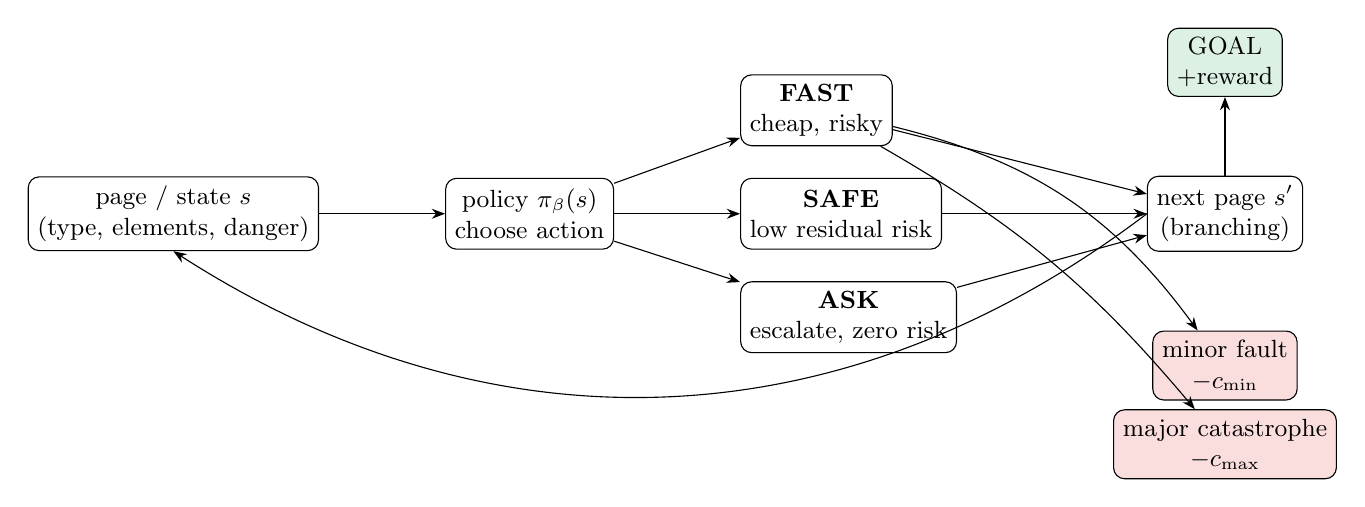
\begin{tikzpicture}[node distance=7mm and 16mm,
  box/.style={draw,rounded corners,align=center,minimum height=9mm,font=\small},
  term/.style={draw,rounded corners,align=center,fill=#1!15,font=\small},
  >={Stealth[]}]
\node[box] (page) {page / state $s$\\(type, elements, danger)};
\node[box,right=of page] (policy) {policy $\pi_\beta(s)$\\choose action};
\node[box,above right=4mm and 16mm of policy] (fast) {\textbf{FAST}\\cheap, risky};
\node[box,right=16mm of policy] (safe) {\textbf{SAFE}\\low residual risk};
\node[box,below right=4mm and 16mm of policy] (ask) {\textbf{ASK}\\escalate, zero risk};
\node[box,right=26mm of safe] (next) {next page $s'$\\(branching)};
\node[term=good,above=10mm of next] (goal) {GOAL\\$+$reward};
\node[term=bad,below=10mm of next] (catm) {minor fault\\$-c_{\min}$};
\node[term=bad,below=20mm of next] (catM) {major catastrophe\\$-c_{\max}$};
\draw[->] (page)--(policy);
\draw[->] (policy)--(fast); \draw[->] (policy)--(safe); \draw[->] (policy)--(ask);
\draw[->] (fast)-- (next); \draw[->] (safe)--(next); \draw[->] (ask)--(next);
\draw[->] (next)--(goal);
\draw[->] (fast) to[bend left=10] (catM);
\draw[->] (fast) to[bend left=20] (catm);
\draw[->] (next.west) to[bend left=35] (page.south);
\end{tikzpicture}}
\caption{The shared decision loop. At each page the risk-sensitive policy chooses
among a cheap-but-risky \textbf{FAST} action, a careful \textbf{SAFE} action, and
an \textbf{ASK} action that escalates to a slow reliable reasoner (System~2).
Risky actions can end in graded failures; reaching the last layer yields the goal
reward.}
\label{fig:flow}
\end{figure}

\begin{description}[leftmargin=1.2em]
\item[RiskyCheckout] a $6$-step linear chain. Rare ($p{=}0.02$) but expensive
  catastrophes with a cost \emph{gradient} across stages ($6,12,20,32,46,64$). A
  minimal setting that isolates the risk effect.
\item[RiskyWeb] a layered \emph{branching} DAG ($8\times3=24$ states) with
  \emph{typed} pages (navigation\,$\ldots$\,payment, confirm) whose danger grows in
  later layers; stochastic branching makes the continuation policy matter.
\item[RiskyFlow] the richest ($10\times4=40$ states): \textbf{graded failures}
  (minor $+$ major catastrophes as separate terminals, so the return distribution
  is heavy-tailed and the three risk measures disagree), \textbf{semantic pages}
  (visible UI elements such as \texttt{confirm\_payment}, \texttt{delete\_account}
  drive danger, so the text is informative), and \textbf{partial observability} (a
  hidden per-page severity modulates danger and is not in the observation --- only
  a noisy hint is). Major-cost range after capping: $[9.6, 90]$.
\end{description}

\section{Experiments and results}

\subsection{Experiment 1 --- the risk ladder (RiskyCheckout)}
We solve the MDP exactly with entropic value iteration over a sweep of $\beta$.
Table~\ref{tab:ladder} shows the per-stage optimal action and
Figure~\ref{fig:risksweep} the resulting outcome statistics.

\begin{table}[H]\centering\small
\caption{RiskyCheckout: optimal action per stage as risk aversion grows. $\beta{=}0$
is ordinary (risk-neutral) Jev value learning.}
\label{tab:ladder}
\begin{tabular}{@{}lll@{}}
\toprule
$\beta$ & per-stage optimal action (stage $1\to6$) & start value $V_0$\\
\midrule
$0.00$ & FAST FAST FAST FAST FAST SAFE & $+9.61$\\
$0.02$ & FAST FAST FAST FAST SAFE SAFE & $+8.61$\\
$0.04$ & FAST FAST FAST SAFE ASK\phantom{A} ASK\phantom{A} & $+7.92$\\
$0.08$ & FAST FAST SAFE ASK\phantom{A} ASK\phantom{A} ASK\phantom{A} & $+6.92$\\
$0.15$ & FAST SAFE ASK\phantom{A} ASK\phantom{A} ASK\phantom{A} ASK\phantom{A} & $+6.33$\\
$0.30$ & SAFE ASK\phantom{A} ASK\phantom{A} ASK\phantom{A} ASK\phantom{A} ASK\phantom{A} & $+5.12$\\
$0.60$ & ASK\phantom{A} ASK\phantom{A} ASK\phantom{A} ASK\phantom{A} ASK\phantom{A} ASK\phantom{A} & $+4.80$\\
\bottomrule
\end{tabular}
\end{table}

\begin{figure}[H]\centering
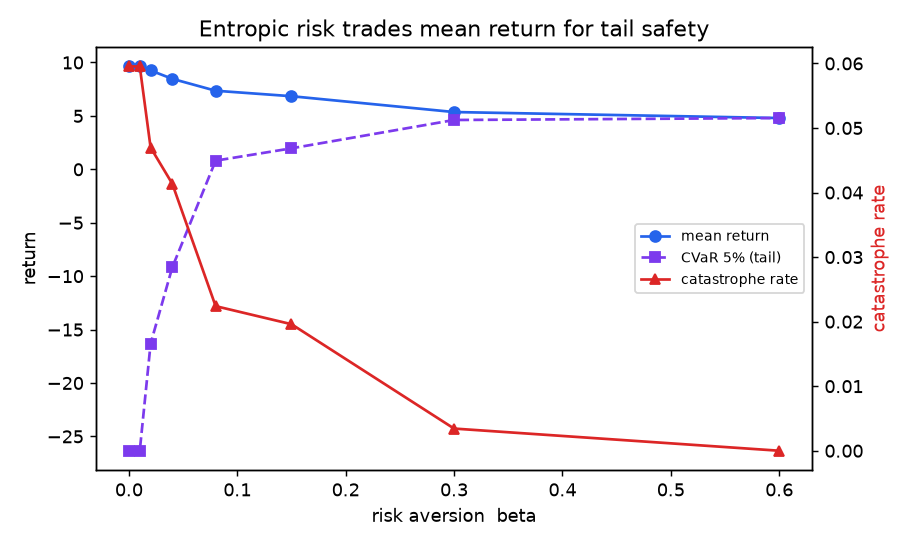
\includegraphics[width=0.72\textwidth]{../results/risk_sweep.png}
\caption{RiskyCheckout outcomes vs $\beta$. As risk aversion grows the policy
drops \textbf{FAST} on the \emph{most expensive} stage first and climbs the ladder
FAST$\to$SAFE$\to$ASK, trading a little mean return for a large reduction in
catastrophe rate and tail risk. Catastrophe rate falls $6\%\to0\%$; worst case
improves from $-46$ to $+4.8$.}
\label{fig:risksweep}
\end{figure}

\paragraph{Takeaway.} Risk neutrality ($\beta{=}0$) uses the fast shortcut almost
everywhere and accepts a $6\%$ catastrophe rate; increasing $\beta$ selectively
avoids the expensive-tail decisions first. The ``ASK'' action realises the blog's
System-1/System-2 hand-off as a first-class, learned behaviour.

\subsection{Experiment 2 --- yev0-4b value head vs baselines (RiskyWeb)}
We train a risk-sensitive value head on frozen \texttt{yev0-4b} features (and, as
an ablation, on MLP features) via entropic fitted value iteration, and compare to
the exact oracle, the risk-neutral policy, and stock \texttt{yev0-4b} used
zero-shot. Table~\ref{tab:web} reports exact metrics at $\beta{=}0.15$;
Figure~\ref{fig:websweep} sweeps $\beta$.

\begin{table}[H]\centering\small
\caption{RiskyWeb at $\beta{=}0.15$. $\Ubeta$ is the entropic objective (higher is
better); ``agree'' is the fraction of states whose action matches the exact oracle.}
\label{tab:web}
\begin{tabular}{@{}lrrrr@{}}
\toprule
policy & mean & catastrophe & $\Ubeta$ & agree \\
\midrule
oracle (entropic VI) & $9.56$ & $0.020$ & $\mathbf{8.01}$ & $1.00$\\
\textbf{yev0-4b + risk head} & $9.56$ & $0.020$ & $\mathbf{8.01}$ & $\mathbf{1.00}$\\
MLP + risk head & $9.56$ & $0.020$ & $8.01$ & $1.00$\\
risk-neutral Jev ($\beta{=}0$) & $\mathbf{11.57}$ & $0.049$ & $-48.31$ & $0.29$\\
stock yev0-4b (zero-shot) & $9.17$ & $0.048$ & $-55.16$ & $0.04$\\
\bottomrule
\end{tabular}
\end{table}

\begin{figure}[H]\centering
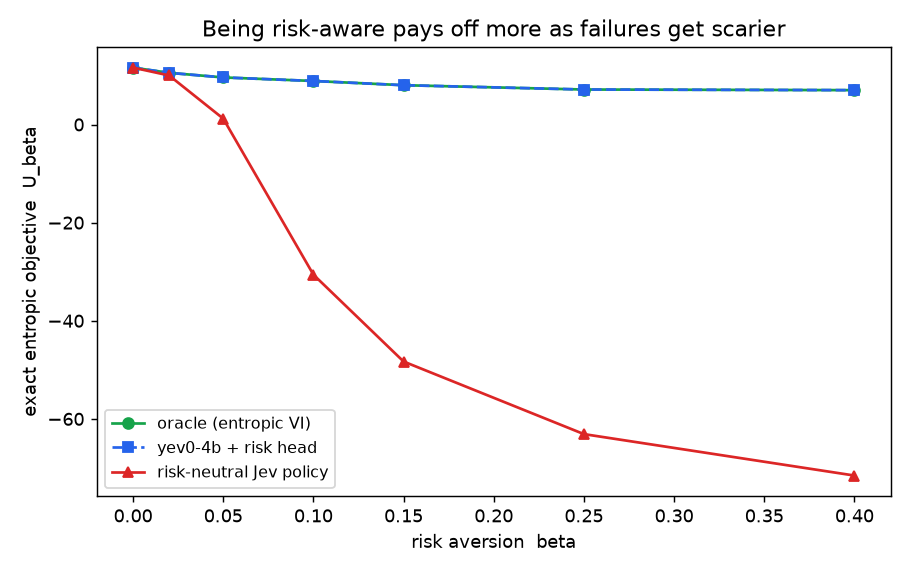
\includegraphics[width=0.72\textwidth]{../results/beta_sweep_web.png}
\caption{RiskyWeb $\beta$ sweep. The value head on \texttt{yev0-4b} features
tracks the exact entropic oracle at \emph{every} risk level (curves coincide,
agreement $1.00$), while the fixed risk-neutral policy's objective collapses from
$11.6$ to $-71.5$ as failures become more fearsome.}
\label{fig:websweep}
\end{figure}

\paragraph{Takeaways.} (i) A risk head trained on \texttt{yev0-4b} features
\emph{recovers the exact risk-sensitive optimum}. (ii) Risk-neutral Jev attains the
\emph{highest mean} ($11.57$) but a catastrophic risk objective ($-48$) --- it
maximises the average while eating a $5\%$ catastrophe rate. (iii) Stock
\texttt{yev0-4b} used zero-shot is risk-blind: a calibrated but risk-neutral model
cannot know your cost structure until a value head is trained on it.

\subsection{Experiment 3 --- full risk-sensitive comparison (RiskyFlow)}
On the richest environment we compare model-based references, model-free learners
(on MLP and on \texttt{yev0-4b} features), heuristics and zero-shot
\texttt{yev0-4b}. Table~\ref{tab:flow} is the headline result (exact metrics,
$\beta{=}0.1$, CVaR $\alpha{=}0.1$), sorted by the entropic objective.

\begin{table}[H]\centering\small
\caption{RiskyFlow comparison, sorted by $\Ubeta$. mean/CVaR/$\Ubeta$ higher is
better; $P(\text{major})$ lower is better. ``agree'' is w.r.t.\ the entropic oracle.}
\label{tab:flow}
\resizebox{\textwidth}{!}{%
\begin{tabular}{@{}lrrrrrr@{}}
\toprule
policy & mean & CVaR & $\Ubeta$ & $P(\text{minor})$ & $P(\text{major})$ & agree\\
\midrule
oracle entropic (VI) & $6.86$ & $2.57$ & $\mathbf{6.31}$ & $0.016$ & $0.0031$ & $1.00$\\
\textbf{yev0-4b finetuned (native, entropic)} & $6.86$ & $2.57$ & $\mathbf{6.31}$ & $0.016$ & $0.0031$ & $\mathbf{1.00}$\\
nested CVaR (DP) & $5.63$ & $\mathbf{4.42}$ & $5.54$ & $0.003$ & $0.0006$ & $0.78$\\
always ASK & $4.98$ & $4.52$ & $4.98$ & $0.000$ & $0.0000$ & $0.75$\\
QR-DQN+CVaR (MLP) & $5.55$ & $2.40$ & $-23.41$ & $0.006$ & $0.0023$ & $0.70$\\
risk-neutral (DP) & $\mathbf{8.45}$ & $-10.93$ & $-39.29$ & $0.059$ & $0.0174$ & $0.47$\\
QR-DQN+CVaR (yev) & $5.20$ & $-1.47$ & $-39.82$ & $0.006$ & $0.0060$ & $0.70$\\
DQN entropic (MLP) & $6.60$ & $-13.24$ & $-49.99$ & $0.033$ & $0.0176$ & $0.78$\\
stock yev0-4b (0-shot) & $6.91$ & $-14.48$ & $-50.47$ & $0.036$ & $0.0192$ & $0.25$\\
always SAFE & $6.54$ & $-24.68$ & $-54.99$ & $0.043$ & $0.0284$ & $0.07$\\
DQN entropic (yev) & $5.04$ & $-33.68$ & $-58.76$ & $0.042$ & $0.0346$ & $0.42$\\
random & $3.72$ & $-53.78$ & $-62.73$ & $0.074$ & $0.0578$ & $0.33$\\
DQN neutral (MLP) & $4.12$ & $-66.55$ & $-63.64$ & $0.096$ & $0.0761$ & $0.17$\\
always FAST & $-1.37$ & $-90.21$ & $-67.51$ & $0.163$ & $0.1272$ & $0.17$\\
\bottomrule
\end{tabular}}
\end{table}

\begin{figure}[H]\centering
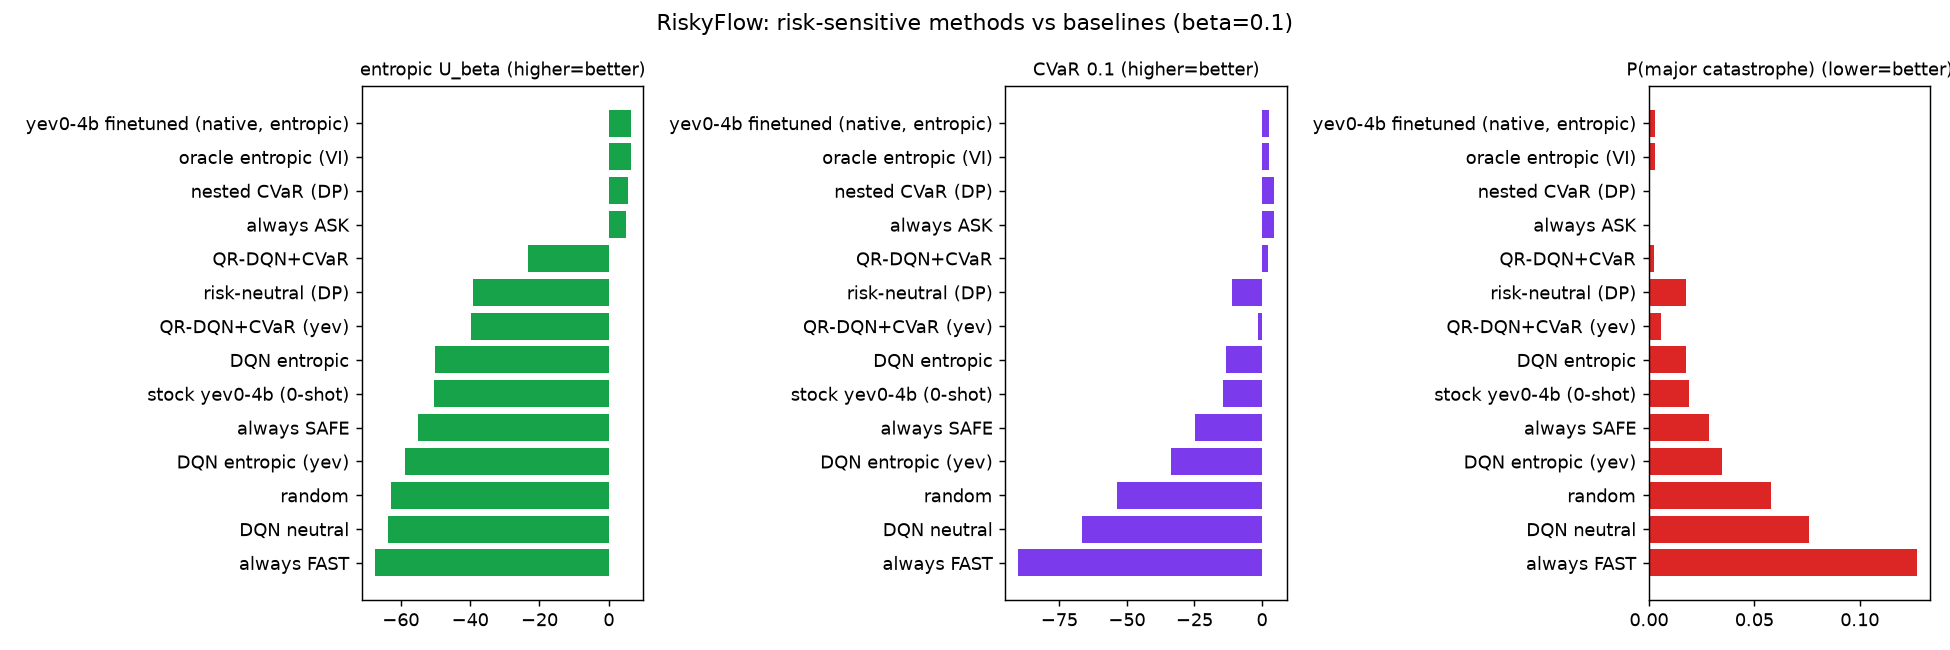
\includegraphics[width=0.93\textwidth]{../results/riskyflow_beta0.1.png}
\caption{RiskyFlow: entropic objective, CVaR and major-catastrophe probability by
method. Risk-sensitive controllers cluster at the top (high $\Ubeta$/CVaR, low
catastrophe); risk-neutral and FAST-leaning policies at the bottom.}
\label{fig:flowbars}
\end{figure}

\begin{figure}[H]\centering
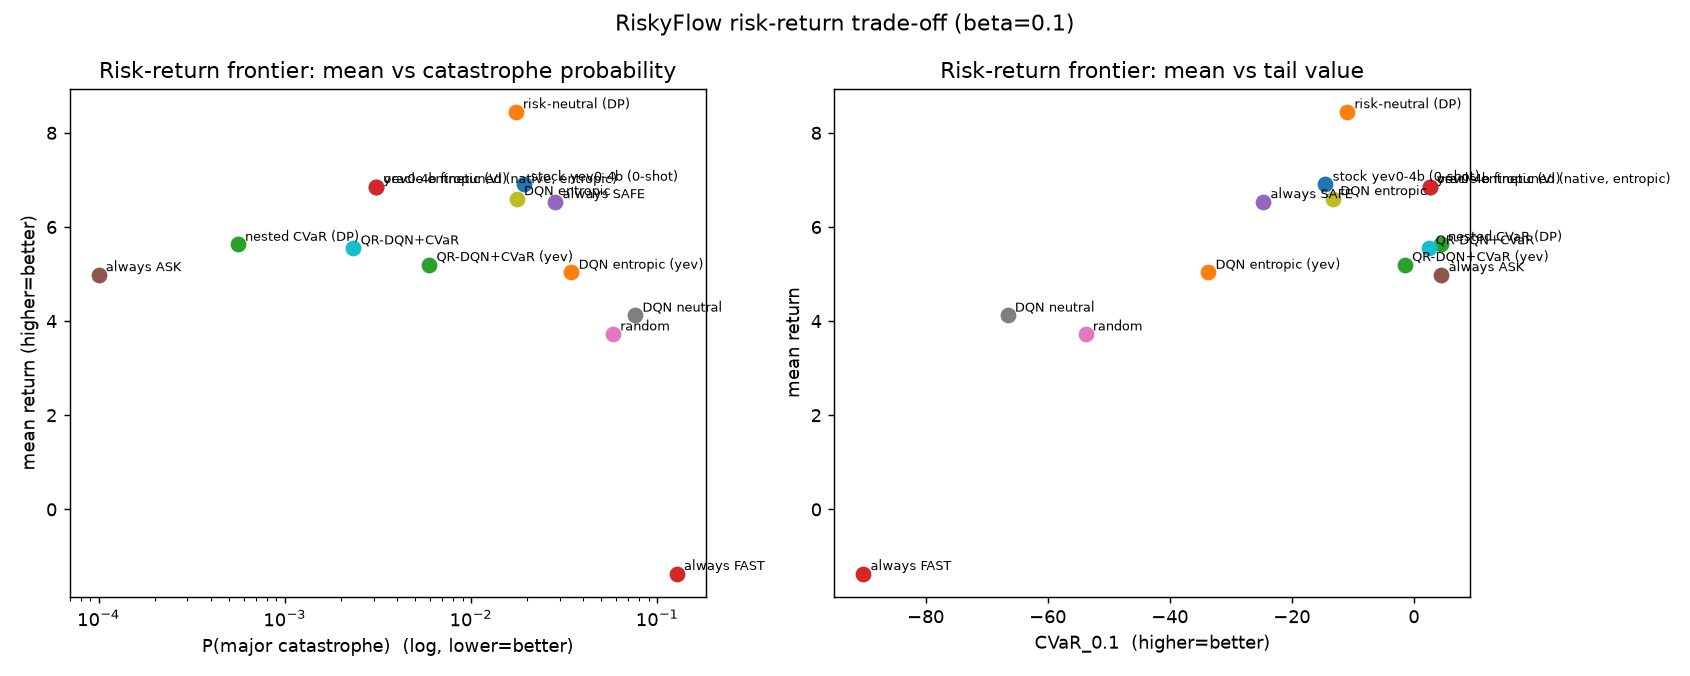
\includegraphics[width=0.95\textwidth]{../results/frontier_beta0.1.png}
\caption{Risk-return frontier. \emph{Left:} mean return vs major-catastrophe
probability (log). \emph{Right:} mean vs CVaR. The risk-neutral DP policy sits at
the highest mean but the worst tail; the entropic oracle, nested CVaR and
\textsc{ask}-leaning policies trade a little mean for a dramatically better tail.}
\label{fig:frontier}
\end{figure}

\begin{figure}[H]\centering
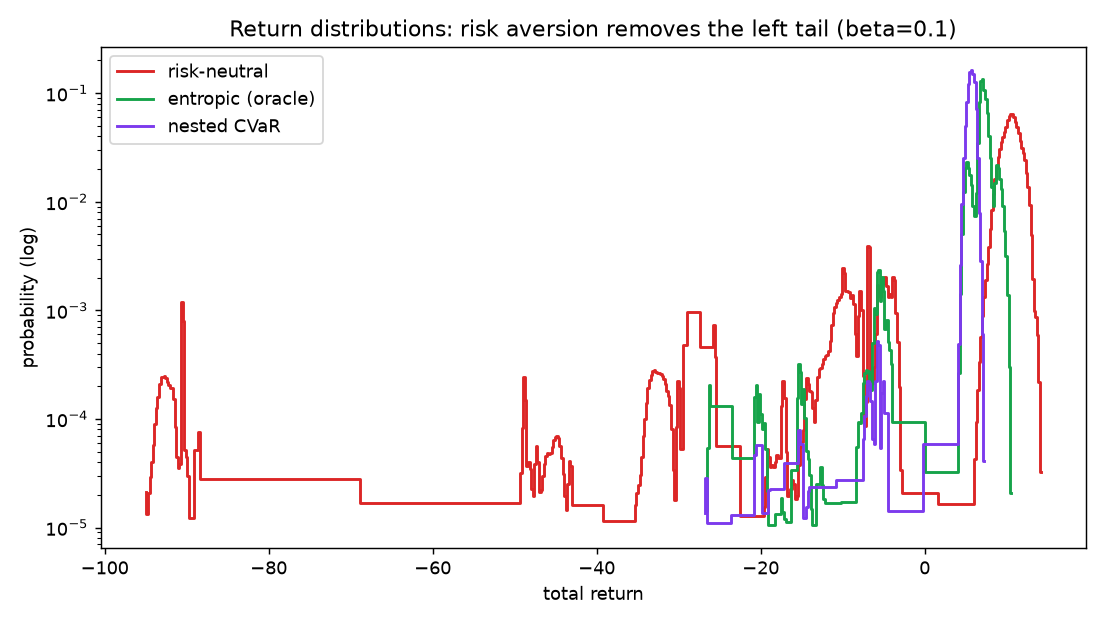
\includegraphics[width=0.72\textwidth]{../results/return_dist_beta0.1.png}
\caption{Return distributions (log scale) of the risk-neutral, entropic-oracle and
nested-CVaR policies. Risk aversion removes probability mass from the deep-negative
left tail (the major catastrophes) at the cost of a slightly lower mode.}
\label{fig:returndist}
\end{figure}

\begin{figure}[H]\centering
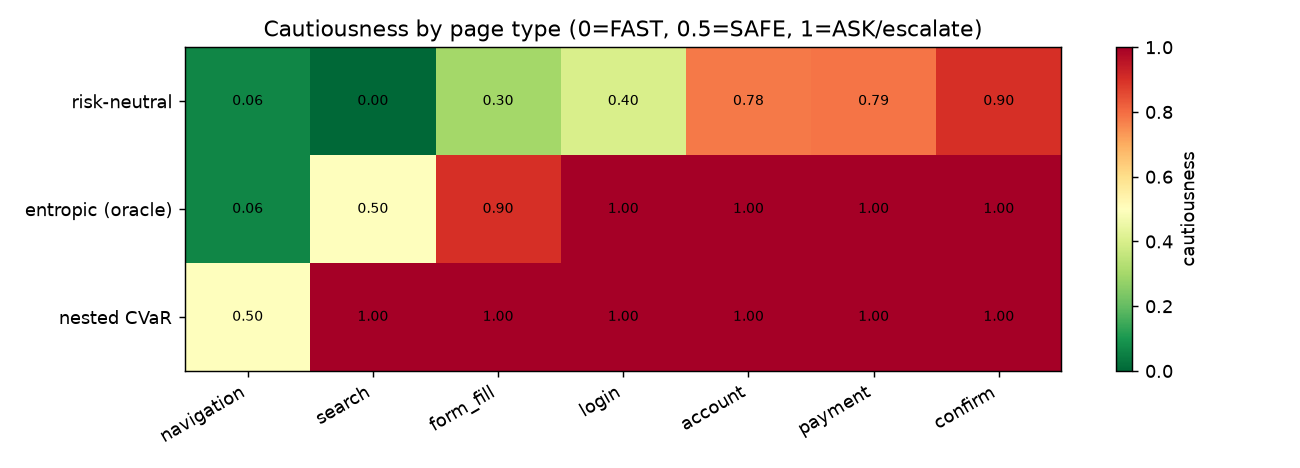
\includegraphics[width=0.92\textwidth]{../results/action_heatmap_beta0.1.png}
\caption{Cautiousness ($0{=}$FAST, $0.5{=}$SAFE, $1{=}$ASK) by page type. The
risk-neutral policy stays fast on most pages; the entropic and CVaR policies
escalate (ASK) precisely on the dangerous page types (payment, confirm, account).}
\label{fig:heatmap}
\end{figure}

\paragraph{Beta sweep.} Sweeping the risk parameter on RiskyFlow
(Table~\ref{tab:flowsweep}, Fig.~\ref{fig:flowsweep}) compares the \emph{adapting}
entropic oracle against the \emph{fixed} risk-neutral and nested-CVaR policies,
scored by $\Ubeta$ and the major-catastrophe rate at each $\beta$. The entropic
oracle keeps a high objective and drives its catastrophe rate to zero as $\beta$
grows, while the risk-neutral policy's objective collapses ($8.45\to-74$) at a
constant $1.7\%$ catastrophe rate; nested CVaR stays tail-safe throughout. The
natively fine-tuned \texttt{yev0-4b} (stars, trained separately at
$\beta\in\{0.05,0.1,0.2\}$) lands \emph{exactly} on the oracle curve at every
$\beta$ tested ($\Ubeta=7.02,6.31,5.23$; agreement $0.97$--$1.00$), confirming that
training yev0-4b's own probabilities recovers the risk-sensitive optimum across
risk levels, not just at a single $\beta$.

\begin{table}[H]\centering\small
\caption{RiskyFlow $\beta$ sweep: entropic objective $\Ubeta$ and major-catastrophe
probability. ``oracle'' adapts to $\beta$; ``r-neutral'' and ``CVaR'' are fixed
policies evaluated at each $\beta$. yev$^\star$ is the natively fine-tuned
\texttt{yev0-4b}.}
\label{tab:flowsweep}
\begin{tabular}{@{}lrrrcrrr@{}}
\toprule
& \multicolumn{3}{c}{$\Ubeta$ (higher better)} & yev$^\star$ &
  \multicolumn{3}{c}{$P(\text{major})$ (lower better)}\\
\cmidrule(lr){2-4}\cmidrule(lr){6-8}
$\beta$ & oracle & r-neutral & CVaR & $\Ubeta$ & oracle & r-neutral & CVaR\\
\midrule
$0.00$ & $8.45$ & $8.45$ & $5.63$ & -- & $0.0174$ & $0.0174$ & $0.0006$\\
$0.05$ & $7.02$ & $-3.67$ & $5.60$ & $7.02$ & $0.0071$ & $0.0174$ & $0.0006$\\
$0.10$ & $6.31$ & $-39.29$ & $5.54$ & $6.31$ & $0.0031$ & $0.0174$ & $0.0006$\\
$0.15$ & $5.69$ & $-56.71$ & $5.42$ & -- & $0.0015$ & $0.0174$ & $0.0006$\\
$0.20$ & $5.23$ & $-65.52$ & $5.10$ & $5.23$ & $0.0005$ & $0.0174$ & $0.0006$\\
$0.30$ & $4.97$ & $-74.38$ & $2.44$ & -- & $0.0000$ & $0.0174$ & $0.0006$\\
\bottomrule
\end{tabular}
\end{table}

\begin{figure}[H]\centering
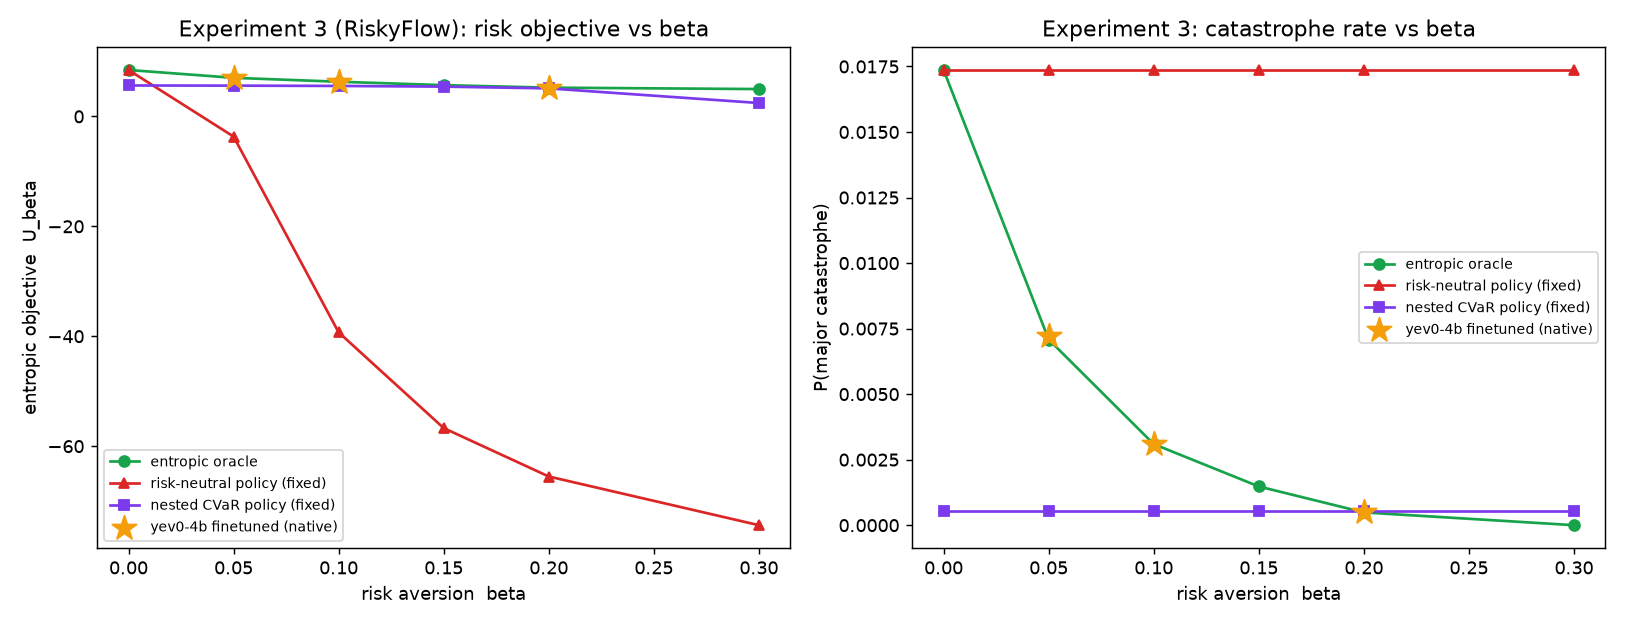
\includegraphics[width=0.95\textwidth]{../results/exp3_beta_sweep.png}
\caption{RiskyFlow ($\beta$ sweep). \emph{Left:} entropic objective $\Ubeta$ --- the
adapting entropic oracle (green) stays high while the fixed risk-neutral policy
(red) collapses; nested CVaR (purple) is stable; natively fine-tuned
\texttt{yev0-4b} (orange stars) sits on the oracle curve. \emph{Right:}
major-catastrophe probability falls to zero for the oracle as $\beta$ grows, while
the risk-neutral policy stays flat.}
\label{fig:flowsweep}
\end{figure}

\paragraph{Takeaways.}
\begin{enumerate}[nosep]
\item The \textbf{model-based risk-sensitive controllers dominate} the risk
  objectives: the entropic oracle has the best $\Ubeta$ and nested CVaR the best
  CVaR, each with a $5$--$10\times$ lower major-catastrophe rate than the
  risk-neutral policy.
\item \textbf{Risk-neutral wins mean only.} The risk-neutral DP policy has the best
  mean ($8.45$) but by far the worst tail among sensible policies
  ($P(\text{major}){=}0.017$, $\Ubeta{=}-39$).
\item \textbf{QR-DQN+CVaR is the best model-free learner} on the tail
  ($P(\text{major}){=}0.0023$, strong CVaR), confirming that model-free tail-risk
  control works here.
\item \textbf{Natively fine-tuned \texttt{yev0-4b} matches the oracle.} Training
  \texttt{yev0-4b}'s \emph{own} Choice probabilities with the blog's log loss
  (Experiment~5, here on RiskyFlow) reaches the \emph{exact} entropic optimum
  ($\Ubeta{=}6.31$, agreement $1.00$, $P(\text{major}){=}0.003$) --- it sits at the
  top of the table alongside the oracle, far above every feature-DQN \texttt{yev}
  variant. Training the model in its native form, against a model-based target, is
  dramatically more effective than model-free learning on raw \texttt{yev} features.
\item \textbf{Honest negatives.} (a) Model-free \emph{entropic} DQN is
  high-variance --- the $\E[e^{-\beta R}]$ estimator has exponentially growing
  variance in $\beta$ --- and did not cut catastrophes as much as the model-based
  entropic oracle. (b) The model-free \emph{DQN} on raw frozen \texttt{yev0-4b}
  hidden features did \emph{not} help (and slightly hurt) versus engineered
  features (Experiment~4); note this is the feature-DQN route, \emph{not} the
  native fine-tuning above, which matches the oracle.
\end{enumerate}

\subsection{Experiment 4 --- do yev0-4b features help the learner?}
\label{sec:sampeff}
We train the entropic DQN on engineered MLP features vs frozen \texttt{yev0-4b}
features across interaction budgets ($500,1500,3000$ episodes, $3$ seeds each) and
evaluate the exact entropic objective and major-catastrophe probability of the
learned policies (Table~\ref{tab:sampeff}, Fig.~\ref{fig:sampeff}).

\begin{table}[H]\centering\small
\caption{Sample efficiency of entropic DQN by feature representation (mean $\pm$ std
over $3$ seeds). Higher $\Ubeta$ and lower $P(\text{major})$ are better. For
reference, the model-based entropic oracle attains $\Ubeta\approx+6.3$.}
\label{tab:sampeff}
\begin{tabular}{@{}lrrrr@{}}
\toprule
& \multicolumn{2}{c}{MLP features} & \multicolumn{2}{c}{yev0-4b features}\\
\cmidrule(lr){2-3}\cmidrule(lr){4-5}
episodes & $\Ubeta$ & $P(\text{major})$ & $\Ubeta$ & $P(\text{major})$\\
\midrule
$500$  & $-27.4\pm22.6$ & $0.016$ & $-54.7\pm 7.9$ & $0.036$\\
$1500$ & $-49.5\pm 1.1$ & $0.024$ & $-25.1\pm26.9$ & $0.012$\\
$3000$ & $-42.2\pm 9.9$ & $0.014$ & $-53.4\pm 1.3$ & $0.022$\\
\bottomrule
\end{tabular}
\end{table}

\begin{figure}[H]\centering
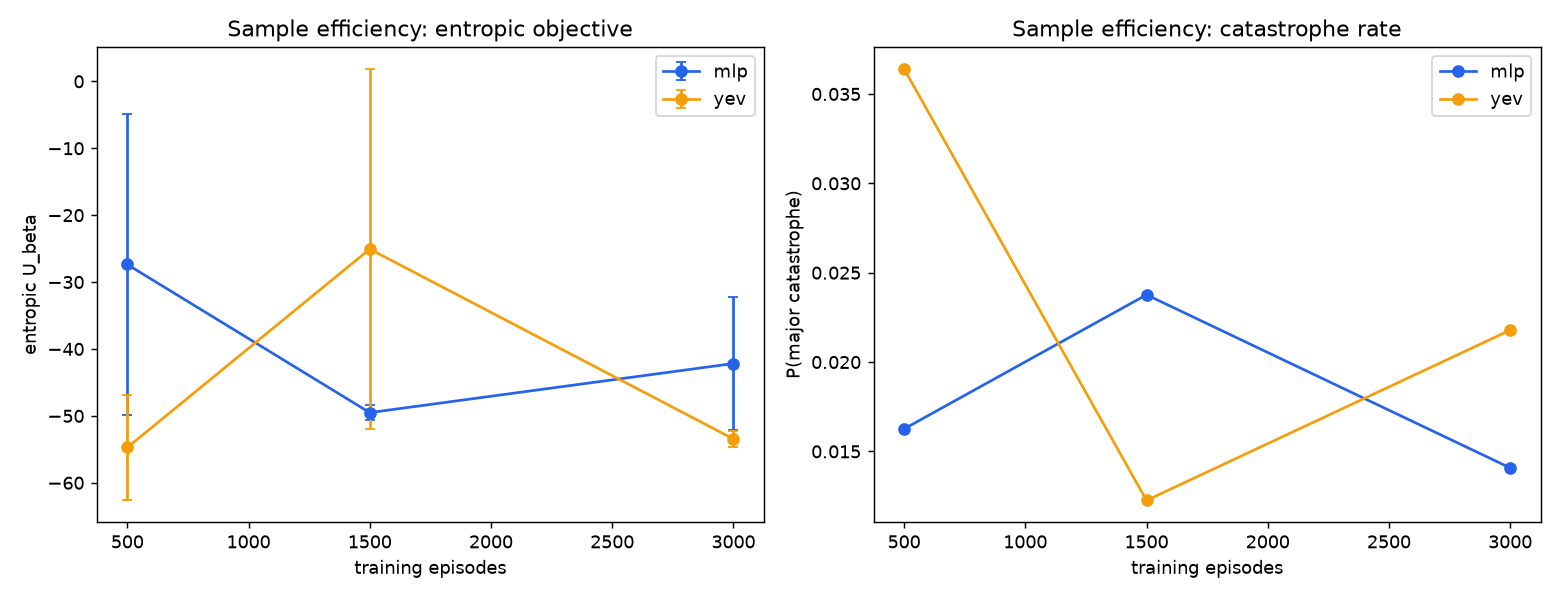
\includegraphics[width=0.92\textwidth]{../results/sample_efficiency.png}
\caption{Sample efficiency of entropic DQN: engineered MLP features vs frozen
\texttt{yev0-4b} features, entropic objective (left) and catastrophe rate (right)
vs training episodes. Error bars are large and the two representations overlap:
there is no consistent advantage to the \texttt{yev0-4b} features here.}
\label{fig:sampeff}
\end{figure}

\paragraph{Takeaway (honest negative).} Neither representation dominates, both are
very noisy (std up to $\pm27$ in $\Ubeta$), and both remain far below the
model-based entropic oracle. The bottleneck is the \emph{estimator}, not the
features: the exponential-utility target $\E[e^{-\beta R}]$ has variance that grows
with $\beta$ and with the catastrophe magnitude, so a single frozen hidden-state
representation does not rescue model-free entropic learning. Representation help, if
any, would more plausibly appear with a lower-variance risk-sensitive estimator
(e.g.\ distributional/IQN) and/or LoRA fine-tuning of the base rather than a frozen
read-out --- a direction we leave to future work.

\subsection{Experiment 5 --- fine-tuning yev0-4b's \emph{native} policy (blog loss)}
\label{sec:finetune}
Experiments 2--4 put a small value \emph{head} on top of \texttt{yev0-4b} features.
Here we instead train \texttt{yev0-4b} \emph{in its original form}: no head is added,
and the policy is read straight off the model's own option-letter distribution (its
Choice readout). We LoRA-fine-tune the base so that this native distribution becomes
the risk-sensitive optimal policy, using the blog's \emph{proper scoring rule} as the
loss --- log loss (cross-entropy) between the model's softmaxed letter logits and the
optimal action distribution from the entropic oracle (Brier gives the same minimiser).
Only LoRA adapters are trained; the base is frozen. This is the faithful analogue of
the blog's ``train $Q_\phi$ with a proper scoring rule'' recipe, applied to
\texttt{yev0-4b}'s own probabilities rather than an external network.

On RiskyWeb at $\beta{=}0.15$ (soft target $\mathrm{softmax}(Q_\beta/\tau)$,
$\tau{=}0.4$, LoRA rank $16$ on all linear layers, $60$ epochs), the log loss falls
$1.24\!\to\!0.26$ and the model's \emph{own} policy becomes the exact
risk-sensitive optimum (Table~\ref{tab:finetune}).

\begin{table}[H]\centering\small
\caption{Fine-tuning yev0-4b's native option probabilities with the blog's log
loss. The policy is read directly from yev0-4b's letter logits (no value head).
``agree'' is the fraction of states matching the entropic oracle.}
\label{tab:finetune}
\begin{tabular}{@{}lrrrr@{}}
\toprule
policy & mean & $\Ubeta$ & $P(\text{cat})$ & agree\\
\midrule
stock yev0-4b (zero-shot) & $9.20$ & $-55.24$ & $0.047$ & $0.04$\\
\textbf{yev0-4b LoRA-finetuned ($\beta{=}0.15$)} & $9.47$ & $\mathbf{+7.94}$ & $0.021$ & $\mathbf{1.00}$\\
oracle entropic (VI) & $9.47$ & $+7.94$ & $0.021$ & $1.00$\\
\bottomrule
\end{tabular}
\end{table}

\paragraph{Takeaway.} Trained \emph{in its original form} --- its own Choice
probabilities, the blog's proper scoring rule --- \texttt{yev0-4b} goes from
risk-blind ($\Ubeta=-55$, $4\%$ agreement with the risk-sensitive oracle) to the
\emph{exact} risk-sensitive optimum ($\Ubeta=+7.94$, $100\%$ agreement), halving the
catastrophe rate, with \emph{no external value head}. This is the cleanest
demonstration of the thesis: the risk attitude is injected purely through the
training target, and the fast decision model's own output carries it. (With a
$\beta{=}0$ target the identical procedure recovers the risk-neutral policy; the
choice of $\beta$ in the target is the only knob.)

\section{Discussion}
The experiments separate two claims that are easy to conflate. First,
\emph{the value is risk-neutral by default}: whether computed exactly, distilled
into a value head, or read zero-shot from \texttt{yev0-4b}, a policy that maximises
expected success quietly accepts rare catastrophes (Tables~\ref{tab:web},
\ref{tab:flow}). Second, \emph{the fix is a change of objective, not of model}: the
same Bellman machinery with the entropic operator (eq.~\ref{eq:entropic-bellman})
produces policies that escalate on exactly the dangerous decisions
(Fig.~\ref{fig:heatmap}) and cut the heavy left tail (Fig.~\ref{fig:returndist}),
and a value head on \texttt{yev0-4b} features recovers this optimum exactly
(Fig.~\ref{fig:websweep}).

The method set also delineates \emph{where} risk-sensitive learning is easy or
hard. Model-based control (value iteration, distributional DP) is exact and cheap
on these tabular problems and gives clean references. Model-free control is harder:
QR-DQN with CVaR selection is a robust tail-risk learner, but the exponential-utility
estimator behind entropic DQN is inherently high-variance, which --- compounded by
partial observability --- keeps it short of the model-based optimum.

\section{Limitations and future work}
\begin{itemize}[nosep]
\item \textbf{Simulation.} All environments are tabular simulators; they are
  designed to isolate the risk phenomenon, not to reproduce a real browser agent.
\item \textbf{Failure costs are specified.} We hand-design the heterogeneous
  catastrophe costs. In a deployment these would have to be elicited or learned,
  which is itself a research question.
\item \textbf{Model-free entropic variance.} A distributional or
  variance-reduced estimator (e.g.\ IQN with an exponential-utility head, or the
  Mihatsch--Neuneier asymmetric-TD surrogate) is the natural next step.
\item \textbf{yev0-4b features.} We used frozen last-layer hidden states with a
  small head. LoRA fine-tuning of the base, or a prompt that better exposes the
  danger semantics, may change the (currently negative) representation result.
\item \textbf{Static vs nested CVaR.} Our CVaR controller is nested; a static-CVaR
  optimiser (augmented-state DP) would be a stronger CVaR reference.
\end{itemize}

\section{Conclusion}
A fast decision model's success probability is an action-value function, and it is
risk-neutral. Making it \emph{risk-sensitive} is a change of objective: replace the
expectation with the entropic risk measure, whose Bellman equation is learnable
from terminal rewards. Across three environments and six learning methods, the
risk-sensitive controllers cut rare-but-costly failures by $5$--$40\times$ at a
small mean-return cost, and a risk-aware router escalates to ``System~2''
precisely on the dangerous decisions. Most directly, LoRA fine-tuning
\texttt{yev0-4b}'s \emph{own} Choice probabilities with the blog's proper scoring
rule makes the model's native output the exact risk-sensitive optimal policy
(Table~\ref{tab:finetune}) --- no external value head --- with the risk attitude
set entirely by the training target $\beta$. This operationalises, and empirically
supports, the blog's hypothesis --- with the added lesson that \emph{how costly a
failure is} must enter the value explicitly, because the probability of success
alone will not reveal it.

\appendix
\section{Reproduction}
From the repository root (conda env with numpy, torch, transformers):
\begin{verbatim}
python -m entropic_risk_jev.src.run_experiment --plot                 # Exp 1
python -m entropic_risk_jev.src.experiment_full --beta 0.15 --device cuda   # Exp 2
python -m entropic_risk_jev.src.sweep_beta --yev --device cuda         # Exp 2 sweep
python -m entropic_risk_jev.src.experiment_v2 --beta 0.1 --device cuda # Exp 3
python -m entropic_risk_jev.src.analysis --beta 0.1                    # extra plots
python -m entropic_risk_jev.src.sample_efficiency --device cuda        # Exp 4
\end{verbatim}

\section{Key hyperparameters}
RiskyFlow: $10\times4$ pages, $\beta{=}0.1$, CVaR $\alpha{=}0.1$, goal reward $15$,
ASK premium $1.0$, SAFE residual-risk factor $0.15$, severity $\in\{0.6,1.0,1.4\}$,
major-cost cap $90$. DQN: $2\times128$ MLP, Adam $10^{-3}$, batch $256$, reward
scale $0.1$, target sync $200$, $4000$ episodes, $\varepsilon$ $1.0\to0.05$.
QR-DQN: $21$ quantiles. Distributional DP: $251$--$601$ atoms. Exact evaluation:
$601$ atoms.

\end{document}
